%%%%%%%%%%%%%%%%%%%%% chapter.tex %%%%%%%%%%%%%%%%%%%%%%%%%%%%%%%%%
%
% sample chapter
%
% Use this file as a template for your own input.
%
%%%%%%%%%%%%%%%%%%%%%%%% Springer-Verlag %%%%%%%%%%%%%%%%%%%%%%%%%%
%\motto{Use the template \emph{chapter.tex} to style the various elements of your chapter content.}

\chapter{Rosetta Code Tasks starting with L}

\section*{LZW compression}

The Lempel-Ziv-Welch (LZW) algorithm provides lossless data compression.
You can read a complete description of it in the
\href{http://en.wikipedia.org/wiki/Lempel-Ziv-Welch}{Wikipedia article}
on the subject. It was patented, but it fell in the public domain in
2004.


\begin{wideverbatim}

(de lzwCompress (Lst)
   (let (Codes 255  Dict)
      (balance 'Dict
         (make
            (for C Codes
               (link (cons (char C) C)) ) ) )
      (make
         (let W (pop 'Lst)
            (for C Lst
               (let WC (pack W C)
                  (if (lup Dict WC)
                     (setq W WC)
                     (link (cdr (lup Dict W)))
                     (idx 'Dict (cons WC (inc 'Codes)) T)
                     (setq W C) ) ) )
            (and W (link (cdr (lup Dict W)))) ) ) ) )

(de lzwDecompress (Lst)
   (let (Codes 255  Dict)
      (balance 'Dict
         (make
            (for C Codes
               (link (list C (char C))) ) ) )
      (make
         (let W NIL
            (for N Lst
               (let WC (if (lup Dict N) (cdr @) (cons (last W) W))
                  (chain (reverse WC))
                  (when W
                     (idx 'Dict (cons (inc 'Codes) (cons (last WC) W)) T) )
                  (setq W WC) ) ) ) ) ) )

Test:

: (lzwCompress (chop "TOBEORNOTTOBEORTOBEORNOT"))
-> (84 79 66 69 79 82 78 79 84 256 258 260 265 259 261 263)

: (pack (lzwDecompress @))
-> "TOBEORNOTTOBEORTOBEORNOT"

\end{wideverbatim}

\pagebreak{}
\section*{Last Fridays of year}

Write a program or a script that returns the last Fridays of each month
of a given year. The year may be given through any simple input method
in your language (command line, std in, etc.).

Example of an expected output:

\begin{verbatim}
./last_fridays 2012
2012-01-27
2012-02-24
2012-03-30
2012-04-27
2012-05-25
2012-06-29
2012-07-27
2012-08-31
2012-09-28
2012-10-26
2012-11-30
2012-12-28
\end{verbatim}

\begin{description}
\item[Cf.]
\end{description}

\begin{itemize}
\item
  \emph{Five weekends}
\item
  \emph{Day of the week}
\end{itemize}


\begin{wideverbatim}

(de lastFridays (Y)
   (for M `(range 1 12)
      (prinl
         (dat\$
            (find '((D) (= "Friday" (day D)))
               (mapcar '((D) (date Y M D)) `(range 31 22)) )
            "-" ) ) ) )

Test:

: (lastFridays 2012)
2012-01-27
2012-02-24
2012-03-30
2012-04-27
2012-05-25
2012-06-29
2012-07-27
2012-08-31
2012-09-28
2012-10-26
2012-11-30
2012-12-28

\end{wideverbatim}

\pagebreak{}
\section*{Last letter-first letter}

A certain childrens game involves starting with a word in a particular
category. Each participant in turn says a word, but that word must begin
with the final letter of the previous word. Once a word has been given,
it cannot be repeated. If an opponent cannot give a word in the
category, they fall out of the game. For example, with ``animals'' as
the category,

\begin{wideverbatim}
Child 1: dog 
Child 2: goldfish
Child 1: hippopotamus
Child 2: snake
...
\end{wideverbatim}

Task Description

Take the following selection of 70 English Pokemon names (extracted from
\href{http://en.wikipedia.org/wiki/List\_of\_Pok\%C3\%A9mon}{Wikipedia's
list of Pokemon}) and generate the/a sequence with the highest possible
number of Pokemon names where the subsequent name starts with the final
letter of the preceding name. No Pokemon name is to be repeated.

\begin{wideverbatim}
audino bagon baltoy banette bidoof braviary bronzor carracosta charmeleon
cresselia croagunk darmanitan deino emboar emolga exeggcute gabite
girafarig gulpin haxorus heatmor heatran ivysaur jellicent jumpluff kangaskhan
kricketune landorus ledyba loudred lumineon lunatone machamp magnezone mamoswine
nosepass petilil pidgeotto pikachu pinsir poliwrath poochyena porygon2
porygonz registeel relicanth remoraid rufflet sableye scolipede scrafty seaking
sealeo silcoon simisear snivy snorlax spoink starly tirtouga trapinch treecko
tyrogue vigoroth vulpix wailord wartortle whismur wingull yamask
\end{wideverbatim}

Extra brownie points for dealing with the full list of 646 names.


\begin{wideverbatim}

(de pokemonChain (File)
   (let Names (make (in File (while (read) (link @))))
      (for Name Names
         (let C (last (chop Name))
            (set Name
               (filter '((Nm) (pre? C Nm)) Names) ) ) )
      (let Res NIL
         (for Name Names
            (let Lst NIL
               (recur (Name Lst)
                  (if (or (memq Name Lst) (not (val (push 'Lst Name))))
                     (when (> (length Lst) (length Res))
                        (setq Res Lst) )
                     (mapc recurse (val Name) (circ Lst)) ) ) ) )
         (flip Res) ) ) )

Test:

: (pokemonChain "pokemon.list")
-> (machamp poliwrath haxorus scrafty yamask kangaskhan nidoking gabite emboar
registeel landorus seaking girafarig gulpin noctowl loudred darmanitan nosepass
simisear rufflet tyrogue exeggcute emolga audino)

: (length @)
-> 24

\end{wideverbatim}

\pagebreak{}
\section*{Leap year}

Determine whether a given year is a leap year in the Gregorian calendar.

\textbf{See Also}

\begin{itemize}
\item
  \href{http://en.wikipedia.org/wiki/Leap\_year}{Leap year (wiki)}
\end{itemize}

\begin{wideverbatim}

(de isLeapYear (Y)
   (bool (date Y 2 29)) )

Output:

: (isLeapYear 2010)
-> NIL

: (isLeapYear 2008)
-> T

: (isLeapYear 1600)
-> T

: (isLeapYear 1700)
-> NIL

\end{wideverbatim}

\pagebreak{}
\section*{Least common multiple}

Compute the least common multiple of two integers.

Given \emph{m} and \emph{n}, the least common multiple is the smallest
positive integer that has both \emph{m} and \emph{n} as factors. For
example, the least common multiple of 12 and 18 is 36, because 12 is a
factor (12 × 3 = 36), and 18 is a factor (18 × 2 = 36), and there is no
positive integer less than 36 that has both factors. As a special case,
if either \emph{m} or \emph{n} is zero, then the least common multiple
is zero.

One way to calculate the least common multiple is to iterate all the
multiples of \emph{m}, until you find one that is also a multiple of
\emph{n}.

If you already have \emph{gcd} for
\emph{greatest common divisor}, then
this formula calculates \emph{lcm}.

\begin{figure}[H]
\centering
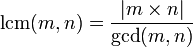
\includegraphics[scale=.6]{graphics/fe9a069fecbc644b6137c76e3dbe21b8.png}
% \caption{\textbackslash{}operatorname\{lcm\}(m, n) =
% \textbackslash{}frac\{\textbar{}m \textbackslash{}times
% n\textbar{}\}\{\textbackslash{}operatorname\{gcd\}(m, n)\}}
\end{figure}

One can also find \emph{lcm} by merging the
\emph{prime decompositions} of both \emph{m}
and \emph{n}.

References:
\href{http://mathworld.wolfram.com/LeastCommonMultiple.html}{MathWorld},
\href{http://en.wikipedia.org/wiki/Least\_common\_multiple}{Wikipedia}.

\begin{wideverbatim}

Using 'gcd' from [[Greatest common divisor#PicoLisp]]:

(de lcm (A B)
   (abs (*/ A B (gcd A B))) )

\end{wideverbatim}

\pagebreak{}
\section*{Letter frequency}

Open a text file and count the occurrences of each letter.

Some of these programs count all characters (including punctuation), but
some only count letters A to Z.


\begin{wideverbatim}

(let Freq NIL
   (in "file.txt"
      (while (char) (accu 'Freq @ 1)) )
   (sort Freq) )

For a "file.txt":

abcd
cdef

Output:

-> (("^J" . 2) ("a" . 1) ("b" . 1) ("c" . 2) ("d" . 2) ("e" . 1) ("f" . 1))

\end{wideverbatim}

\pagebreak{}
\section*{Levenshtein distance}

In information theory and computer science, the \textbf{Levenshtein
distance} is a
\href{http://en.wikipedia.org/wiki/string\_metric}{metric} for measuring
the amount of difference between two sequences (i.e. an
\href{http://en.wikipedia.org/wiki/edit\_distance}{edit distance}). The
Levenshtein distance between two strings is defined as the minimum
number of edits needed to transform one string into the other, with the
allowable edit operations being insertion, deletion, or substitution of
a single character.

For example, the Levenshtein distance between "\textbf{kitten}" and
"\textbf{sitting}" is 3, since the following three edits change one into
the other, and there is no way to do it with fewer than three edits:

\begin{enumerate}
\item
  \textbf{k}itten \textbf{s}itten (substitution of `k' with 's')
\item
  sitt\textbf{e}n sitt\textbf{i}n (substitution of `e' with `i')
\item
  sittin sittin\textbf{g} (insert `g' at the end).
\end{enumerate}

\emph{The Levenshtein distance between
  "\textbf{rosettacode}``,''\textbf{raisethysword}" is 8; The distance
  between two strings is same as that when both strings is reversed.}

\textbf{Task~:} Implements a Levenshtein distance function, or uses a
library function, to show the Levenshtein distance between ``kitten''
and ``sitting''.

\textbf{Other edit distance at Rosettacode.org}~:

\begin{itemize}
\item
  \emph{Longest common subsequence}

\begin{wideverbatim}

(de levenshtein (A B)
   (let D
      (cons
         (range 0 (length A))
         (mapcar
            '((I) (cons I (copy A)))
            (range 1 (length B)) ) )
      (for (J . Y) B
         (for (I . X) A
            (set
               (nth D (inc J) (inc I))
               (if (= X Y)
                  (get D J I)
                  (inc
                     (min
                        (get D J (inc I))
                        (get D (inc J) I)
                        (get D J I) ) ) ) ) ) ) ) )

or, using 'map' to avoid list indexing:

(de levenshtein (A B)
   (let D
      (cons
         (range 0 (length A))
         (mapcar
            '((I) (cons I (copy A)))
            (range 1 (length B)) ) )
      (map
         '((B Y)
            (map
               '((A X P)
                  (set (cdr P)
                     (if (= (car A) (car B))
                        (car X)
                        (inc (min (cadr X) (car P) (car X))) ) ) )
               A
               (car Y)
               (cadr Y) ) )
         B
         D ) ) )

Output in both cases:

: (levenshtein (chop "kitten") (chop "sitting"))
-> 3

\end{wideverbatim}

\pagebreak{}
\section*{Linear congruential generator}

The
\href{http://en.wikipedia.org/wiki/linear\_congruential\_generator}{linear
  congruential generator} is a very simple example of a \emph{random
  number generator}. All linear congruential generators use this
formula:

\begin{itemize}
\item
  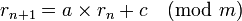
\includegraphics[scale=.6]{graphics/25e1b8e2f59974728e2a729ad51ba0bd.png}
\end{itemize}

Where:

\begin{itemize}
\item
  \emph{r}\textsubscript{0} is a seed.
\item
  \emph{r}\textsubscript{1}, \emph{r}\textsubscript{2},
  \emph{r}\textsubscript{3}, \ldots{}, are the random numbers.
\item
  \emph{a}, \emph{c}, \emph{m} are constants.
\end{itemize}

If one chooses the values of \emph{a}, \emph{c} and \emph{m} with care,
then the generator produces a uniform distribution of integers from 0 to
\emph{m} − 1.

LCG numbers have poor quality. \emph{r}\textsubscript{\emph{n}} and
\emph{r}\textsubscript{\emph{n} + 1} are not independent, as true random
numbers would be. Anyone who knows \emph{r}\textsubscript{\emph{n}} can
predict \emph{r}\textsubscript{\emph{n} + 1}, therefore LCG is not
cryptographically secure. The LCG is still good enough for simple tasks
like \emph{Miller-Rabin primality
test}, or \emph{FreeCell deals}. Among
the benefits of the LCG, one can easily reproduce a sequence of numbers,
from the same \emph{r}\textsubscript{0}. One can also reproduce such
sequence with a different programming language, because the formula is
so simple.

The task is to replicate two historic random number generators. One is
the \texttt{rand()} function from \emph{BSD
libc}, and the other is the \texttt{rand()} function from the Microsoft
C Runtime (MSCVRT.DLL). Each replica must yield the same sequence of
integers as the original generator, when starting from the same seed.

In these formulas, the seed becomes
\emph{s}\emph{t}\emph{a}\emph{t}\emph{e}\textsubscript{0}. The random
sequence is \emph{r}\emph{a}\emph{n}\emph{d}\textsubscript{1},
\emph{r}\emph{a}\emph{n}\emph{d}\textsubscript{2} and so on.

BSD formula:

\begin{itemize}
\item
  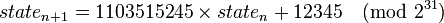
\includegraphics[scale=.6]{graphics/8c943c1cc7df75afeddd50d9ad93e28e.png}
\item
  \emph{r}\emph{a}\emph{n}\emph{d}\textsubscript{\emph{n}} =
  \emph{s}\emph{t}\emph{a}\emph{t}\emph{e}\textsubscript{\emph{n}}
\item
  \emph{r}\emph{a}\emph{n}\emph{d}\textsubscript{\emph{n}} is in range 0
  to 2147483647.
\end{itemize}

Microsoft formula:

\begin{itemize}
\item
  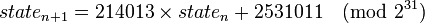
\includegraphics[scale=.6]{graphics/c9f11575eec8aadcac4687458ded5aa3.png}
\item
  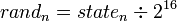
\includegraphics[scale=.6]{graphics/a026db06e1a9bd6945c85c8e17231725.png}
\item
  \emph{r}\emph{a}\emph{n}\emph{d}\textsubscript{\emph{n}} is in range 0
  to 32767.
\end{itemize}

The BSD formula was so awful that FreeBSD switched to a different
formula. More info is at \emph{Random number generator (included)\#C}.

\begin{wideverbatim}

(zero *BsdSeed *MsSeed)

(de bsdRand ()
   (setq *BsdSeed
      (\& (+ 12345 (* 1103515245 *BsdSeed)) `(dec (** 2 31))) ) )

(de msRand ()
   (>> 16
      (setq *MsSeed
         (\& (+ 2531011 (* 214013 *MsSeed)) `(dec (** 2 31))) ) ) )

Output:

: (do 7 (printsp (bsdRand)))
12345 1406932606 654583775 1449466924 229283573 1109335178 1051550459 -> 1051550459

: (do 12 (printsp (msRand)))
38 7719 21238 2437 8855 11797 8365 32285 10450 30612 5853 28100 -> 28100

\end{wideverbatim}

\pagebreak{}
\section*{List comprehensions}

A \href{http://en.wikipedia.org/wiki/List\_comprehension}{list
comprehension} is a special syntax in some programming languages to
describe lists. It is similar to the way mathematicians describe sets,
with a \emph{set comprehension}, hence the name.

Some attributes of a list comprehension are that:

\begin{enumerate}
\item
  They should be distinct from (nested) for loops within the syntax of
  the language.
\item
  They should return either a list or an iterator (something that
  returns successive members of a collection, in order).
\item
  The syntax has parts corresponding to that of
  \href{http://en.wikipedia.org/wiki/Set-builder\_notation}{set-builder
  notation}.
\end{enumerate}

Write a list comprehension that builds the list of all
\emph{Pythagorean triples} with elements between 1 and n. If the
language has multiple ways for expressing such a construct (for
example, direct list comprehensions and generators), write one example
for each.

\begin{wideverbatim}

PicoLisp doesn't have list comprehensions.
We might use a generator function, pipe, coroutine or pilog predicate.

# Using a generator function

(de pythag (N)
   (job '((X . 1) (Y . 1) (Z . 0))
      (loop
         (when (> (inc 'Z) N)
            (when (> (inc 'Y) N)
               (setq Y (inc 'X)) )
            (setq Z Y) )
         (T (> X N))
         (T (= (+ (* X X) (* Y Y)) (* Z Z))
            (list X Y Z) ) ) ) )

(while (pythag 20)
   (println @) )

# Using a pipe

(pipe
   (for X 20
      (for Y (range X 20)
         (for Z (range Y 20)
            (when (= (+ (* X X) (* Y Y)) (* Z Z))
               (pr (list X Y Z)) ) ) ) )
   (while (rd)
      (println @) ) )

# Using a coroutine

Coroutines are available only in the 64-bit version.

(de pythag (N)
   (co 'pythag
      (for X N
         (for Y (range X N)
            (for Z (range Y N)
               (when (= (+ (* X X) (* Y Y)) (* Z Z))
                  (yield (list X Y Z)) ) ) ) ) ) )

(while (pythag 20)
   (println @) )

\end{wideverbatim}

\begin{wideverbatim}

Output in all three cases:

(3 4 5)
(5 12 13)
(6 8 10)
(8 15 17)
(9 12 15)
(12 16 20)

# Using Pilog

{{works with|PicoLisp|3.0.9.7}}

(be pythag (@N @X @Y @Z)
   (for @X @N)
   (for @Y @X @N)
   (for @Z @Y @N)
   (@ let (X (-> @X)  Y (-> @Y)  Z (-> @Z))
       (= (+ (* X X) (* Y Y)) (* Z Z)) ) )


Test:

: (? (pythag 20 @X @Y @Z))
 @X=3 @Y=4 @Z=5
 @X=5 @Y=12 @Z=13
 @X=6 @Y=8 @Z=10
 @X=8 @Y=15 @Z=17
 @X=9 @Y=12 @Z=15
 @X=12 @Y=16 @Z=20
-> NIL

\end{wideverbatim}

\pagebreak{}
\section*{Literals/Floating point}

Programming languages have different ways of expressing floating-point
literals. Show how floating-point literals can be expressed in your
language: decimal or other bases, exponential notation, and any other
special features.

You may want to include a regular expression or BNF/ABNF/EBNF defining
allowable formats for your language.

See also \emph{Literals/Integer}.

\begin{wideverbatim}

PicoLisp does not support floating point literals in the base language, only
fixed point (scaled) decimal integers of unlimited size and precision. See
[http://software-lab.de/doc/ref.html#num-io Numbers] in the reference.

\end{wideverbatim}

\pagebreak{}
\section*{Literals/Integer}

Some programming languages have ways of expressing integer literals in
bases other than the normal base ten.

Show how integer literals can be expressed in as many bases as your
language allows.

Note: this should \textbf{not} involve the calling of any
functions/methods but should be interpreted by the compiler or
interpreter as an integer written to a given base.

Also show any other ways of expressing literals, e.g. for different
types of integers.

See also \emph{Literals/Floating point}.

Cf. \emph{Extreme floating point
values}

\begin{wideverbatim}

In the strict sense of this task, PicoLisp reads only integers at bases which
are a power of ten (scaled fixpoint numbers). This is controlled via the global
variable '[http://software-lab.de/doc/refS.html#*Scl *Scl]':

: (setq *Scl 4)
-> 4

: 123.456789
-> 1234568

However, the reader is normally augmented by read macros, which can read any
base or any desired format. Read macros are not executed at runtime, but
intially when the sources are read.

: '(a `(hex "7F") b `(oct "377") c)
-> (a 127 b 255 c)

In addition to standard formats like
'[http://software-lab.de/doc/refH.html#hex hex]' (hexadecimal) and
'[http://software-lab.de/doc/refO.html#oct oct]' (octal),
there are also more esoteric formats like
'[http://software-lab.de/doc/refF.html#fmt64 fmt64]' (base 64) and
'[http://software-lab.de/doc/refH.html#hax hax]' (hexadecimal numbers
coded with alphabetic characters).

\end{wideverbatim}

\pagebreak{}
\section*{Literals/String}


Show literal specification of characters and strings. If supported, show
how verbatim strings (quotes where escape sequences are quoted
literally) and here-strings work. Also, discuss which quotes expand
variables.

\begin{itemize}
\item
  Related tasks: \emph{Special characters},
  \emph{Here document}
\end{itemize}



\begin{wideverbatim}

PicoLisp doesn't have a string data type. Instead, symbols are used. Certain
uninterned symbols, called
[http://software-lab.de/doc/ref.html#transient "transient symbols"],
however, look and behave like strings on other languages.

Syntactically, transient symbols (called "strings" in the following)  are
surrounded by double quotes.

: "ab\"cd"
-> "ab\"cd"

Double quotes in strings are escaped with a backslash.

ASCII control characters can be written using the hat ('^') character:

: "ab^Icd^Jef"  # Tab, linefeed

There is no special character type or representation. Individual characters are
handled as single-character strings:

: (chop "abc")
-> ("a" "b" "c")

: (pack (reverse @))
-> "cba"

A limited handling of here-strings is available with the
'[http://software-lab.de/doc/refH.html#here here]' function.

\end{wideverbatim}

\pagebreak{}
\section*{Logical operations}

\textbf{Basic Data Operation}\\ This is a basic data operation. It
represents a fundamental action on a basic data type.

You may see other such operations in the \emph{Basic Data Operations}
category, or:

\textbf{Integer Operations} \\
\emph{Arithmetic} \textbar{} \emph{Comparison}

\textbf{Boolean Operations} \\ \emph{Bitwise} \textbar{}
\textbf{Logical}

\textbf{String Operations} \\
\emph{Concatenation} \textbar{} \emph{Interpolation} \textbar{}
\emph{Matching}

\textbf{Memory Operations} \\
\emph{Pointers \& references} \textbar{} \emph{Addresses}

Write a function that takes two logical (boolean) values, and outputs
the result of ``and'' and ``or'' on both arguments as well as ``not'' on
the first arguments. If the programming language doesn't provide a
separate type for logical values, use the type most commonly used for
that purpose.

If the language supports additional logical operations on booleans such
as XOR, list them as well.

\begin{wideverbatim}

(de logic (A B)
   (prin "A AND B is ")
   (println (and A B))
   (prin "A OR B is ")
   (println (or A B))
   (prin "A XOR B is ")
   (println (xor A B))
   (prin "NOT A is ")
   (println (not A)) )

\end{wideverbatim}

\pagebreak{}
\section*{Long multiplication}

In this task, explicitly implement
\href{http://en.wikipedia.org/wiki/long\_multiplication}{long
multiplication}. This is one possible approach to arbitrary-precision
integer algebra.

For output, display the result of 2\^{}64 * 2\^{}64. The decimal
representation of 2\^{}64 is:

\begin{verbatim}
18446744073709551616
\end{verbatim}

The output of 2\^{}64 * 2\^{}64 is 2\^{}128, and that is:

\begin{verbatim}
340282366920938463463374607431768211456
\end{verbatim}

\begin{wideverbatim}

: (* (** 2 64) (** 2 64))
-> 340282366920938463463374607431768211456

\end{wideverbatim}

\pagebreak{}
\section*{Longest common subsequence}

The \textbf{longest common subsequence} (or \textbf{LCS}) of groups A
and B is the longest group of elements from A and B that are common
between the two groups and in the same order in each group. For example,
the sequences ``1234'' and ``1224533324'' have an LCS of ``1234'':

\begin{verbatim}
1234
1224533324
\end{verbatim}

For a string example, consider the sequences ``thisisatest'' and
``testing123testing''. An LCS would be ``tsitest'':

\begin{verbatim}
thisisatest
testing123testing
\end{verbatim}

In this puzzle, your code only needs to deal with strings. Write a
function which returns an LCS of two strings (case-sensitive). You don't
need to show multiple LCS's.

For more information on this problem please see
\href{http://en.wikipedia.org/wiki/Longest\_common\_subsequence\_problem}{Wikipedia}.

\begin{wideverbatim}

(de commonSequences (A B)
   (when A
      (conc
         (when (member (car A) B)
            (mapcar '((L) (cons (car A) L))
               (cons NIL (commonSequences (cdr A) (cdr @))) ) )
         (commonSequences (cdr A) B) ) ) )

(maxi length
   (commonSequences
      (chop "thisisatest")
      (chop "testing123testing") ) )

Output:

-> ("t" "s" "i" "t" "e" "s" "t")

\end{wideverbatim}

\pagebreak{}
\section*{Longest string challenge}

\textbf{Background}

This problem and challenge is inspired by one that used to be given as a
challenge to students learning Icon. It was intended to be tried in Icon
and another language the student was familiar with. The basic problem is
quite simple the challenge and fun part came through the introduction of
restrictions. Experience has shown that the original restrictions
required some adjustment to bring out the intent of the challenge and
make it suitable for Rosetta Code.

The original programming challenge and some solutions can be found at
\href{https://tapestry.tucson.az.us/twiki/bin/view/Main/LongestStringsPuzzle}{Unicon
Programming TWiki / Longest Strings Puzzle}. (See notes on talk page if
you have trouble with the site).

\textbf{Basic problem statement:}

Write a program that reads lines from standard input and, upon end of
file, writes the longest line to standard output.

If there are ties for the longest line, the program writes out all the
lines that tie.

If there is no input, the program should produce no output.

\textbf{Task}

Implement a solution to the basic problem that adheres to the spirit of
the restrictions (see below).

Describe how you circumvented or got around these `restrictions' and met
the `spirit' of the challenge. Your supporting description may need to
describe any challenges to interpreting the restrictions and how you
made this interpretation. You should state any assumptions, warnings, or
other relevant points. The central idea here is to make the task a bit
more interesting by thinking outside of the box and perhaps show off the
capabilities of your language in a creative way. Because there is
potential for more variation between solutions, the description is key
to helping others see what you've done.

This task is likely to encourage multiple different types of solutions.
They should be substantially different approaches.

Given the input:

\begin{verbatim}
a
bb
ccc
ddd
ee
f
ggg
\end{verbatim}

The output should be (possibly rearranged):

\begin{verbatim}
ccc
ddd
ggg
\end{verbatim}

\textbf{Original list of restrictions:}

1. No comparison operators may be used.

2. No arithmetic operations, such as addition and subtraction, may be
used.

3. The only datatypes you may use are integer and string. In particular,
you may not use lists.

An additional restriction became apparent in the discussion.

4. Do not re-read the input file. Avoid using files as a replacement for
lists.

\textbf{Intent of Restrictions}

Because of the variety of languages on Rosetta and the wide variety of
concepts used in them there needs to be a bit of clarification and
guidance here to get to the spirit of the challenge and the intent of
the restrictions.

The basic problem can be solved very conventionally and that's boring
and pedestrian. The original intent here wasn't to unduly frustrate
people with interpreting the restrictions, it was to get people to think
outside of their particular box and have a bit of fun doing it.

The guiding principle here should be that when using the language of
your choice, try to solve this creatively showing off some of your
language capabilities. If you need to bend the restrictions a bit,
explain why and try to follow the intent. If you think you've
implemented a `cheat' call out the fragment yourself and ask the reader
if they can spot why. If you absolutely can't get around one of the
restrictions, say why in your description.

Now having said that, the restrictions require some elaboration.

\begin{itemize}
\item
  In general, the restrictions are meant to avoid the explicit use of
  these features.
\item
  ``No comparison operators may be used'' - At some level there must be
  some test that allows the solution to get at the length and determine
  if one string is longer. Comparison operators, in particular any
  less/greater comparison should be avoided. Representing the length of
  any string as a number should also be avoided. Various approaches
  allow for detecting the end of a string. Some of these involve
  implicitly using equal/not-equal; however, explicitly using
  equal/not-equal should be acceptable.
\item
  ``No arithmetic operations'' - Again, at some level something may have
  to advance through the string. Often there are ways a language can do
  this implicitly advance a cursor or pointer without explicitly using a
  +, - , ++, --, add, subtract, etc.
\item
  The datatype restrictions are amongst the most difficult to
  reinterpret. In the language of the original challenge strings are
  atomic datatypes and structured datatypes like lists are quite
  distinct and have many different operations that apply to them. This
  becomes a bit fuzzier with languages with a different programming
  paradigm. The intent would be to avoid using an easy structure to
  accumulate the longest strings and spit them out. There will be some
  natural reinterpretation here.
\end{itemize}

To make this a bit more concrete, here are a couple of specific
examples:

In C, a string is an array of chars, so using a couple of arrays as
strings is in the spirit while using a second array in a non-string like
fashion would violate the intent.

In APL or J, arrays are the core of the language so ruling them out is
unfair. Meeting the spirit will come down to how they are used.

Please keep in mind these are just examples and you may hit new
territory finding a solution. There will be other cases like these.
Explain your reasoning. You may want to open a discussion on the talk
page as well.

\begin{itemize}
\item
  The added ``No rereading'' restriction is for practical reasons,
  re-reading stdin should be broken. I haven't outright banned the use
  of other files but I've discouraged them as it is basically another
  form of a list. Somewhere there may be a language that just sings when
  doing file manipulation and where that makes sense; however, for most
  there should be a way to accomplish without resorting to an
  externality.
\end{itemize}

At the end of the day for the implementer this should be a bit of fun.
As an implementer you represent the expertise in your language, the
reader may have no knowledge of your language. For the reader it should
give them insight into how people think outside the box in other
languages. Comments, especially for non-obvious (to the reader) bits
will be extremely helpful. While the implementations may be a bit
artificial in the context of this task, the general techniques may be
useful elsewhere.

\begin{wideverbatim}

Not sure if this meets the spirit. I would implement it the same way if there
were no "restrictions":

(mapc prinl
   (maxi '((L) (length (car L)))
      (by length group
         (in NIL
            (make (until (eof) (link (line)))) ) ) ) )

Another solution avoids 'group', and builds an associative buffer of lines
instead:

(let Buf NIL
   (in NIL
      (until (eof)
         (let (Line (line)  Len (length Line))
            (if (assoc Len Buf)
               (conc @ (cons Line))
               (push 'Buf (cons Len (cons Line))) ) ) ) )
   (mapc prinl (cdr (maxi car Buf))) )

\end{wideverbatim}

\pagebreak{}
\section*{Look-and-say sequence}

\textbf{Sequence Definition}

\begin{itemize}
\item
  Take a decimal number
\item
  \emph{Look} at the number, visually grouping consecutive runs of the
  same digit.
\item
  \emph{Say} the number, from left to right, group by group; as how many
  of that digit there are - followed by the digit grouped.
\end{itemize}

This becomes the next number of the sequence.

The
\href{http://en.wikipedia.org/wiki/Look\_and\_say\_sequence}{sequence}
is from \href{http://en.wikipedia.org/wiki/John\_Horton\_Conway}{John
Conway}, of \emph{Conway's Game of
Life} fame.

\textbf{An example:}

\begin{itemize}
\item
  Starting with the number 1, you have \emph{one} 1 which produces 11.
\item
  Starting with 11, you have \emph{two} 1's i.e. 21
\item
  Starting with 21, you have \emph{one} 2, then \emph{one} 1 i.e.
  (12)(11) which becomes 1211
\item
  Starting with 1211 you have \emph{one} 1, \emph{one} 2, then
  \emph{two} 1's i.e. (11)(12)(21) which becomes 111221
\end{itemize}

\textbf{Task description}

Write a program to generate successive members of the look-and-say
sequence.

\textbf{See also}

\begin{itemize}
\item
  This task is related to, and an application of, the
  \emph{Run-length encoding} task.
\end{itemize}


\begin{wideverbatim}

(de las (Lst)
   (make
      (while Lst
         (let (N 1  C)
            (while (= (setq C (pop 'Lst)) (car Lst))
               (inc 'N) )
            (link N C) ) ) ) )

Usage:

: (las (1))
-> (1 1)
: (las @)
-> (2 1)
: (las @)
-> (1 2 1 1)
: (las @)
-> (1 1 1 2 2 1)
: (las @)
-> (3 1 2 2 1 1)
: (las @)
-> (1 3 1 1 2 2 2 1)
: (las @)
-> (1 1 1 3 2 1 3 2 1 1)
: (las @)
-> (3 1 1 3 1 2 1 1 1 3 1 2 2 1)

\end{wideverbatim}

\pagebreak{}
\section*{Loop over multiple arrays simultaneously}


Loop over multiple arrays (or lists or tuples or whatever they're called
in your language) and print the \emph{i}th element of each. Use your
language's ``for each'' loop if it has one, otherwise iterate through
the collection in order with some other loop.

For this example, loop over the arrays \texttt{(a,b,c)},
\texttt{(A,B,C)} and \texttt{(1,2,3)} to produce the output

\begin{verbatim}
aA1
bB2
cC3
\end{verbatim}

If possible, also describe what happens when the arrays are of different
lengths.



\begin{wideverbatim}

(mapc prinl
   '(a b c)
   '(A B C)
   (1 2 3) )

The length of the first argument list controls the operation. If subsequent
lists are longer, their remaining values are ignored. If they are shorter, NIL
is passed to the function.

\end{wideverbatim}

\pagebreak{}
\section*{Loops/Break}

Show a loop which prints random numbers (each number newly generated
each loop) from 0 to 19 (inclusive). If a number is 10, stop the loop
after printing it, and do not generate any further numbers. Otherwise,
generate and print a second random number before restarting the loop. If
the number 10 is never generated as the first number in a loop, loop
forever.

\begin{wideverbatim}

Literally:

(use R
   (loop
      (println (setq R (rand 1 19)))
      (T (= 10 R))
      (println (rand 1 19)) ) )

Shorter:

(until (= 10 (println (rand 1 19)))
   (println (rand 1 19)) )

\end{wideverbatim}

\pagebreak{}
\section*{Loops/Continue}

Show the following output using one loop.

\begin{verbatim}
1, 2, 3, 4, 5
6, 7, 8, 9, 10
\end{verbatim}

Try to achieve the result by forcing the next iteration within the loop
upon a specific condition, if your language allows it.


\begin{wideverbatim}

PicoLisp doesn't have an explicit 'continue' functionality. It can always be
emulated with a conditional expression.

(for I 10
   (print I)
   (if (=0 (\% I 5))
      (prinl)
      (prin ", ") ) )

\end{wideverbatim}

\pagebreak{}
\section*{Loops/Do-while}

Start with a value at 0. Loop while value mod 6 is not equal to 0. Each
time through the loop, add 1 to the value then print it. The loop must
execute at least once.

\begin{wideverbatim}

Literally:

(let Val 0
   (loop
      (println (inc 'Val))
      (T (=0 (\% Val 6))) ) )

Shorter:

(let Val 0
   (until (=0 (\% (println (inc 'Val)) 6))) )

or:

(for (Val 0  (n0 (\% (println (inc 'Val)) 6))))

\end{wideverbatim}

\pagebreak{}
\section*{Loops/Downward for}

Write a for loop which writes a countdown from 10 to 0.

\begin{wideverbatim}

(for (I 10 (ge0 I) (dec I))
   (println I) )

or:

(mapc println (range 10 0))

\end{wideverbatim}

\pagebreak{}
\section*{Loops/For}

``For'' loops are used to make some block of code be iterated a number
of times, setting a variable or parameter to a monotonically increasing
integer value for each execution of the block of code. Common extensions
of this allow other counting patterns or iterating over abstract
structures other than the integers.

For this task, show how two loops may be nested within each other, with
the number of iterations performed by the inner for loop being
controlled by the outer for loop. Specifically print out the following
pattern by using one for loop nested in another:

\begin{verbatim}
*
**
***
****
*****
\end{verbatim}


\begin{wideverbatim}

(for N 5
   (do N (prin "*"))
   (prinl) )

\end{wideverbatim}

\pagebreak{}
\section*{Loops/For with a specified step}

Demonstrate a for loop where the step value is greater than one.

\begin{wideverbatim}

(for (N 1 (> 10 N) (+ N 2))
   (printsp N) )

\end{wideverbatim}

\pagebreak{}
\section*{Loops/Foreach}

Loop through and print each element in a collection in order. Use your
language's ``for each'' loop if it has one, otherwise iterate through
the collection in order with some other loop.


\begin{wideverbatim}

(mapc println '(Apple Banana Coconut))

\end{wideverbatim}

\pagebreak{}
\section*{Loops/Infinite}

Specifically print out ``SPAM'' followed by a newline in an infinite
loop.

\begin{wideverbatim}

(loop (prinl "SPAM"))

\end{wideverbatim}

\pagebreak{}
\section*{Loops/N plus one half}

Quite often one needs loops which, in the last iteration, execute only
part of the loop body. The goal of this task is to demonstrate the best
way to do this.

Write a loop which writes the comma-separated list

\begin{verbatim}
1, 2, 3, 4, 5, 6, 7, 8, 9, 10
\end{verbatim}

using separate output statements for the number and the comma from
within the body of the loop.

See also: \emph{Loop/Break}

\begin{wideverbatim}

(for N 10
   (prin N)
   (T (= N 10))
   (prin ", ") )

\end{wideverbatim}

\pagebreak{}
\section*{Loops/Nested}

Show a nested loop which searches a two-dimensional array filled with
random numbers uniformly distributed over
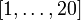
\includegraphics[scale=.6]{graphics/31b36ed3111d6cf3e8fa29c9ef59a501.png}.
The loops iterate rows and columns of the array printing the elements
until the value 20 is met. Specifically, this task also shows how to
\emph{break} out of nested loops.

\begin{wideverbatim}

(for Lst (make (do 10 (link (make (do 10 (link (rand 1 20)))))))
   (T
      (for N Lst
         (printsp N)
         (T (= N 20) T) ) ) )

or:

(catch NIL
   (for Lst (make (do 10 (link (make (do 10 (link (rand 1 20)))))))
      (for N Lst
         (printsp N)
         (and (= N 20) (throw)) ) ) )

\end{wideverbatim}

\pagebreak{}
\section*{Loops/While}

Start an integer value at 1024. Loop while it is greater than 0. Print
the value (with a newline) and divide it by two each time through the
loop.

\begin{wideverbatim}

(let N 1024
   (while (gt0 N)
      (println N)
      (setq N (/ N 2)) ) )

\end{wideverbatim}

\pagebreak{}
\section*{Lucas-Lehmer test}


Lucas-Lehmer Test: for \emph{p} an odd prime, the Mersenne number
2\textsuperscript{\emph{p}} − 1 is prime if and only if
2\textsuperscript{\emph{p}} − 1 divides \emph{S}(\emph{p} − 1) where
\emph{S}(\emph{n} + 1) = (\emph{S}(\emph{n}))\textsuperscript{2} − 2,
and \emph{S}(1) = 4.

The following programs calculate all Mersenne primes up to the
implementation's maximum precision, or the 47th Mersenne prime. (Which
ever comes first).



\begin{wideverbatim}

(de prime? (N)
   (or
      (= N 2)
      (and
         (> N 1)
         (bit? 1 N)
         (for (D 3  T  (+ D 2))
            (T (> D (sqrt N)) T)
            (T (=0 (\% N D)) NIL) ) ) ) )

(de mersenne? (P)
   (or
      (= P 2)
      (let (MP (dec (>> (- P) 1))  S 4)
         (do (- P 2)
            (setq S (\% (- (* S S) 2) MP)) )
         (=0 S) ) ) )

Output:

: (for N 10000
   (and (prime? N) (mersenne? N) (println N)) )
2
3
5
7
13
17
19
31
61
89
107
127
521
607
1279
2203
2281
3217
4253
4423
9689
9941

\end{wideverbatim}

\pagebreak{}
\section*{Luhn test of credit card numbers}


The \href{http://en.wikipedia.org/wiki/Luhn\_algorithm}{Luhn test} is
used by some credit card companies to distinguish valid credit card
numbers from what could be a random selection of digits.

Those companies using credit card numbers that can be validated by the
Luhn test have numbers that pass the following test:

\begin{enumerate}
\item
  Reverse the order of the digits in the number.
\item
  Take the first, third, \ldots{} and every other odd digit in the
  reversed digits and sum them to form the partial sum s1
\item
  Taking the second, fourth \ldots{} and every other even digit in the
  reversed digits:
\end{enumerate}

\begin{enumerate}
\item
  Multiply each digit by two and sum the digits if the answer is greater
  than nine to form partial sums for the even digits
\item
  Sum the partial sums of the even digits to form s2
\end{enumerate}

\begin{enumerate}
\item
  If s1 + s2 ends in zero then the original number is in the form of a
  valid credit card number as verified by the Luhn test.
\end{enumerate}

For example, if the trial number is 49927398716:

\begin{wideverbatim}
Reverse the digits:
  61789372994
Sum the odd digits:
  6 + 7 + 9 + 7 + 9 + 4 = 42 = s1
The even digits:
    1,  8,  3,  2,  9
  Two times each even digit:
    2, 16,  6,  4, 18
  Sum the digits of each multiplication:
    2,  7,  6,  4,  9
  Sum the last:
    2 + 7 + 6 + 4 + 9 = 28 = s2

s1 + s2 = 70 which ends in zero 
which means that 49927398716 passes the Luhn test
\end{wideverbatim}


\pagebreak{}

The task is to \textbf{write a function/method/procedure/subroutine that
will validate a number with the Luhn test, and use it to validate the
following numbers:}

49927398716

49927398717

1234567812345678

1234567812345670

Cf. \emph{SEDOL}



\begin{wideverbatim}

(de luhn (Num)  # 'Num' may be a number or a string
   (=0
      (\%
         (sum
            '((C F)
               (setq C (- (char C) 48))
               (if F
                  C                               # Odd
                  (+ (/ C 5) (\% (* 2 C) 10)) ) )  # Even
            (flip (chop Num))
            '(T NIL .) )
         10 ) ) )

Output:

: (mapcar luhn (49927398716 49927398717 1234567812345678 1234567812345670))
-> (0 NIL NIL 0)

\end{wideverbatim}



% %%%%%%%%%%%%%%%%%%%%%%%% referenc.tex %%%%%%%%%%%%%%%%%%%%%%%%%%%%%%
% sample references
% %
% Use this file as a template for your own input.
%
%%%%%%%%%%%%%%%%%%%%%%%% Springer-Verlag %%%%%%%%%%%%%%%%%%%%%%%%%%
%
% BibTeX users please use
% \bibliographystyle{}
% \bibliography{}
%
\biblstarthook{In view of the parallel print and (chapter-wise) online publication of your book at \url{www.springerlink.com} it has been decided that -- as a genreral rule --  references should be sorted chapter-wise and placed at the end of the individual chapters. However, upon agreement with your contact at Springer you may list your references in a single seperate chapter at the end of your book. Deactivate the class option \texttt{sectrefs} and the \texttt{thebibliography} environment will be put out as a chapter of its own.\\\indent
References may be \textit{cited} in the text either by number (preferred) or by author/year.\footnote{Make sure that all references from the list are cited in the text. Those not cited should be moved to a separate \textit{Further Reading} section or chapter.} The reference list should ideally be \textit{sorted} in alphabetical order -- even if reference numbers are used for the their citation in the text. If there are several works by the same author, the following order should be used: 
\begin{enumerate}
\item all works by the author alone, ordered chronologically by year of publication
\item all works by the author with a coauthor, ordered alphabetically by coauthor
\item all works by the author with several coauthors, ordered chronologically by year of publication.
\end{enumerate}
The \textit{styling} of references\footnote{Always use the standard abbreviation of a journal's name according to the ISSN \textit{List of Title Word Abbreviations}, see \url{http://www.issn.org/en/node/344}} depends on the subject of your book:
\begin{itemize}
\item The \textit{two} recommended styles for references in books on \textit{mathematical, physical, statistical and computer sciences} are depicted in ~\cite{science-contrib, science-online, science-mono, science-journal, science-DOI} and ~\cite{phys-online, phys-mono, phys-journal, phys-DOI, phys-contrib}.
\item Examples of the most commonly used reference style in books on \textit{Psychology, Social Sciences} are~\cite{psysoc-mono, psysoc-online,psysoc-journal, psysoc-contrib, psysoc-DOI}.
\item Examples for references in books on \textit{Humanities, Linguistics, Philosophy} are~\cite{humlinphil-journal, humlinphil-contrib, humlinphil-mono, humlinphil-online, humlinphil-DOI}.
\item Examples of the basic Springer style used in publications on a wide range of subjects such as \textit{Computer Science, Economics, Engineering, Geosciences, Life Sciences, Medicine, Biomedicine} are ~\cite{basic-contrib, basic-online, basic-journal, basic-DOI, basic-mono}. 
\end{itemize}
}

\begin{thebibliography}{99.}%
% and use \bibitem to create references.
%
% Use the following syntax and markup for your references if 
% the subject of your book is from the field 
% "Mathematics, Physics, Statistics, Computer Science"
%
% Contribution 
\bibitem{science-contrib} Broy, M.: Software engineering --- from auxiliary to key technologies. In: Broy, M., Dener, E. (eds.) Software Pioneers, pp. 10-13. Springer, Heidelberg (2002)
%
% Online Document
\bibitem{science-online} Dod, J.: Effective substances. In: The Dictionary of Substances and Their Effects. Royal Society of Chemistry (1999) Available via DIALOG. \\
\url{http://www.rsc.org/dose/title of subordinate document. Cited 15 Jan 1999}
%
% Monograph
\bibitem{science-mono} Geddes, K.O., Czapor, S.R., Labahn, G.: Algorithms for Computer Algebra. Kluwer, Boston (1992) 
%
% Journal article
\bibitem{science-journal} Hamburger, C.: Quasimonotonicity, regularity and duality for nonlinear systems of partial differential equations. Ann. Mat. Pura. Appl. \textbf{169}, 321--354 (1995)
%
% Journal article by DOI
\bibitem{science-DOI} Slifka, M.K., Whitton, J.L.: Clinical implications of dysregulated cytokine production. J. Mol. Med. (2000) doi: 10.1007/s001090000086 
%
\bigskip

% Use the following (APS) syntax and markup for your references if 
% the subject of your book is from the field 
% "Mathematics, Physics, Statistics, Computer Science"
%
% Online Document
\bibitem{phys-online} J. Dod, in \textit{The Dictionary of Substances and Their Effects}, Royal Society of Chemistry. (Available via DIALOG, 1999), 
\url{http://www.rsc.org/dose/title of subordinate document. Cited 15 Jan 1999}
%
% Monograph
\bibitem{phys-mono} H. Ibach, H. L\"uth, \textit{Solid-State Physics}, 2nd edn. (Springer, New York, 1996), pp. 45-56 
%
% Journal article
\bibitem{phys-journal} S. Preuss, A. Demchuk Jr., M. Stuke, Appl. Phys. A \textbf{61}
%
% Journal article by DOI
\bibitem{phys-DOI} M.K. Slifka, J.L. Whitton, J. Mol. Med., doi: 10.1007/s001090000086
%
% Contribution 
\bibitem{phys-contrib} S.E. Smith, in \textit{Neuromuscular Junction}, ed. by E. Zaimis. Handbook of Experimental Pharmacology, vol 42 (Springer, Heidelberg, 1976), p. 593
%
\bigskip
%
% Use the following syntax and markup for your references if 
% the subject of your book is from the field 
% "Psychology, Social Sciences"
%
%
% Monograph
\bibitem{psysoc-mono} Calfee, R.~C., \& Valencia, R.~R. (1991). \textit{APA guide to preparing manuscripts for journal publication.} Washington, DC: American Psychological Association.
%
% Online Document
\bibitem{psysoc-online} Dod, J. (1999). Effective substances. In: The dictionary of substances and their effects. Royal Society of Chemistry. Available via DIALOG. \\
\url{http://www.rsc.org/dose/Effective substances.} Cited 15 Jan 1999.
%
% Journal article
\bibitem{psysoc-journal} Harris, M., Karper, E., Stacks, G., Hoffman, D., DeNiro, R., Cruz, P., et al. (2001). Writing labs and the Hollywood connection. \textit{J Film} Writing, 44(3), 213--245.
%
% Contribution 
\bibitem{psysoc-contrib} O'Neil, J.~M., \& Egan, J. (1992). Men's and women's gender role journeys: Metaphor for healing, transition, and transformation. In B.~R. Wainrig (Ed.), \textit{Gender issues across the life cycle} (pp. 107--123). New York: Springer.
%
% Journal article by DOI
\bibitem{psysoc-DOI}Kreger, M., Brindis, C.D., Manuel, D.M., Sassoubre, L. (2007). Lessons learned in systems change initiatives: benchmarks and indicators. \textit{American Journal of Community Psychology}, doi: 10.1007/s10464-007-9108-14.
%
%
% Use the following syntax and markup for your references if 
% the subject of your book is from the field 
% "Humanities, Linguistics, Philosophy"
%
\bigskip
%
% Journal article
\bibitem{humlinphil-journal} Alber John, Daniel C. O'Connell, and Sabine Kowal. 2002. Personal perspective in TV interviews. \textit{Pragmatics} 12:257--271
%
% Contribution 
\bibitem{humlinphil-contrib} Cameron, Deborah. 1997. Theoretical debates in feminist linguistics: Questions of sex and gender. In \textit{Gender and discourse}, ed. Ruth Wodak, 99--119. London: Sage Publications.
%
% Monograph
\bibitem{humlinphil-mono} Cameron, Deborah. 1985. \textit{Feminism and linguistic theory.} New York: St. Martin's Press.
%
% Online Document
\bibitem{humlinphil-online} Dod, Jake. 1999. Effective substances. In: The dictionary of substances and their effects. Royal Society of Chemistry. Available via DIALOG. \\
http://www.rsc.org/dose/title of subordinate document. Cited 15 Jan 1999
%
% Journal article by DOI
\bibitem{humlinphil-DOI} Suleiman, Camelia, Daniel C. O�Connell, and Sabine Kowal. 2002. `If you and I, if we, in this later day, lose that sacred fire...�': Perspective in political interviews. \textit{Journal of Psycholinguistic Research}. doi: 10.1023/A:1015592129296.
%
%
%
\bigskip
%
%
% Use the following syntax and markup for your references if 
% the subject of your book is from the field 
% "Computer Science, Economics, Engineering, Geosciences, Life Sciences"
%
%
% Contribution 
\bibitem{basic-contrib} Brown B, Aaron M (2001) The politics of nature. In: Smith J (ed) The rise of modern genomics, 3rd edn. Wiley, New York 
%
% Online Document
\bibitem{basic-online} Dod J (1999) Effective Substances. In: The dictionary of substances and their effects. Royal Society of Chemistry. Available via DIALOG. \\
\url{http://www.rsc.org/dose/title of subordinate document. Cited 15 Jan 1999}
%
% Journal article by DOI
\bibitem{basic-DOI} Slifka MK, Whitton JL (2000) Clinical implications of dysregulated cytokine production. J Mol Med, doi: 10.1007/s001090000086
%
% Journal article
\bibitem{basic-journal} Smith J, Jones M Jr, Houghton L et al (1999) Future of health insurance. N Engl J Med 965:325--329
%
% Monograph
\bibitem{basic-mono} South J, Blass B (2001) The future of modern genomics. Blackwell, London 
%
\end{thebibliography}

